\subsection{Benchmarks}
\label{subsec:benchmark}

\paragraph{Frequency of Updates}
To determine the frequency of updates, values received per second where averaged over 100 seconds, although the data from the first and last second were ignored due to the potential of partial data.
The rate of updates from the gyroscope is very steady, at about 31.6 Updates per second.
The frequency of new values from the ultrasonic sensor is not as steady, as it depends on the distance being measured.
This is because longer distances take longer to measure, and the arduino immediately starts a new measurement upon completion. Figure \ref{fig:benchmark} shows a plot of the measured values, also presented in Table \ref{table:benchmark}.

\begin{table}
    \centering
    \begin{tabular}{l|lll}
            & Measured Distance & Gyroscope & Ultrasound \\
        \cline{1-3}
        10  & 10.33490          & 31.54639  & 602.1531   \\
        20  & 20.25844          & 31.59596  & 441.9388   \\
        30  & 30.32993          & 31.59184  & 347.5556   \\
        50  & 50.38063          & 31.59794  & 252.7551   \\
        75  & 75.66509          & 31.60204  & 187.5859   \\
        100 & 99.08760          & 31.60204  & 147.4949   \\
        150 & 150.85837         & 31.60204  & 103.9596   \\
        200 & 203.61689         & 31.60825  & 79.0102    \\
    \end{tabular}

    \caption{Expected and measured distance in cm from sensor and update frequency of sensors, average over 100 seconds}
    \label{table:benchmark}
\end{table}

\begin{figure}
    \centering
    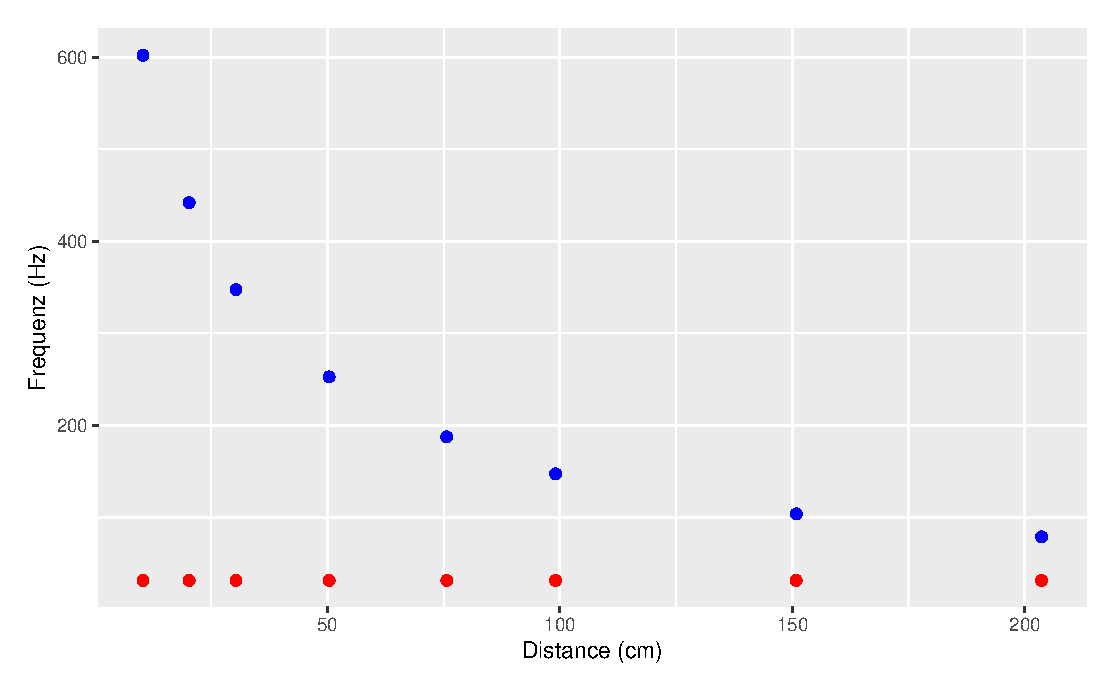
\includegraphics[width=0.5\linewidth]{figures/benchmark.eps}
    \caption{The data from \ref{table:benchmark} visualized}
    \label{fig:benchmark}
\end{figure}

